\section{Conceptual Foundations of Microservice Architectures and their Interfaces}\label{sec:foundations}

\subsection{Microservices and Microservice Architectures}

Microservices and Microservice Architectures are a widely adopted architectural style originating from \acp{SOA}~\cite{Mazzara2020}.
In contrast to \ac{SOA}, microservices do not primarily focus on reuse and composition, but on independence, replaceability, and autonomy~\cite{Baresi2020}.
Building an application using a microservice architecture describes the approach of decomposing the application into a set of small services (so-called \textit{microservices}), each running in their own process, providing a lightweight way of interacting with each other, often using \ac{HTTP} and \ac{REST}~\cite{Lewis2014}.
One service is responsible for a business capability.
Services can be deployed independently and in an automated fashion.

Enterprise applications typically consist of a client-side \ac{UI}, a database, and a server-side application~\cite{Lewis2014}.
The server-side application handles user requests, executes domain logic, queries and updates the database, and populates views for the user.
Traditional applications following the monolithic architectural style package this functionality into a single logical executable, such that updates to any parts of the system require rebuilding and redeployment of the whole system.
Structuring this application only happens via language features such as classes, functions, and namespaces.
Horizontally scaling this application requires running multiple instances of the application behind a load-balancer.
While modularization can also be achieved with this monolithic style, microservices make the separation of modules explicit, by running in their own process.
They also allow scaling only the parts of the application requiring more resources.

According to Lewis and Fowler~\cite{Lewis2014}, there is no formal definition of microservice architecture, but common characteristics of the style can be identified.
However, not all microservice architectures will have all the characteristics, but most of them will exhibit most of the characteristics.

\paragraph{Componentization via Services}

Microservice architectures use services as their primary componentization mechanism~\cite{Lewis2014}.
Componentization via libraries and software modules can be called with in-memory function calls.
This contrasts out-of-process services, where communication is more expensive, as it requires using a mechanism such as web service requests, or \acp{RPC}.
However, this also makes services independently deployable (see \autoref{fig:ms-componentization:mic}), whereas applications linked to a single executable must be built and deployed as a whole (see \autoref{fig:ms-componentization:mon}).
As a result, this allows better utilizing available resources as the parts of the application experiencing higher load can be horizontally scaled.
Additionally, changes to a service only require this service to be redeployed in most cases, while the rest of the application remains running.
Only changes to the interface of a service may require coordination between multiple services, however, this can also be avoided by cohesive service boundaries and evolution mechanisms in the service contracts.
However, having explicit service contracts requiring remote \ac{API} calls make it harder to breaking encapsulation than in-process function calls.

\begin{figure}[!htb]
    \centering
    \begin{subfigure}{.5\textwidth}
        \centering
        \begin{tikzpicture}[
    node distance=3cm,
    process/.style = {
        draw,
        rectangle
    },
    functionality/.style = {
        draw,
        circle,
        minimum width = 5mm
    },
    server/.style = {
        draw,
        rectangle
    },
    sline/.style = {
        line cap=round,
        line join=round
    }
]

\node[functionality, color=theme1, fill=theme1!10] (f1) {};
\node[functionality, right=3mm of f1, color=theme2, fill=theme2!10] (f2) {};
\node[functionality, below=3mm of f1, color=theme3, fill=theme3!10] (f3) {};
\node[functionality, right=3mm of f3, color=theme4, fill=theme4!10] (f4) {};
\node[process, fit=(f1)(f2)(f3)(f4)] (proc1) {};
\node[above=0 of proc1] (l1) {Process};
\node[server, fit=(proc1)(l1)] (srv1) {};
\draw[sline, fill=black!5] (srv1.north west) -- ++(0.25,0.25) -- ($(srv1.north east)+(0.25,0.25)$) -- (srv1.north east);
\draw[sline, fill=black!10] (srv1.north east) -- ++(0.25,0.25) -- ($(srv1.south east)+(0.25,0.25)$) -- (srv1.south east);
\node[below=0 of srv1] (l2) {Server A};


\node[functionality, right=2cm of f2, color=theme1, fill=theme1!10] (f5) {};
\node[functionality, right=3mm of f5, color=theme2, fill=theme2!10] (f6) {};
\node[functionality, below=3mm of f5, color=theme3, fill=theme3!10] (f7) {};
\node[functionality, right=3mm of f7, color=theme4, fill=theme4!10] (f8) {};
\node[process, fit=(f5)(f6)(f7)(f8)] (proc2) {};
\node[above=0 of proc2] (l3) {Process};
\node[server, fit=(proc2)(l3)] (srv2) {};
\draw[sline, fill=black!5] (srv2.north west) -- ++(0.25,0.25) -- ($(srv2.north east)+(0.25,0.25)$) -- (srv2.north east);
\draw[sline, fill=black!10] (srv2.north east) -- ++(0.25,0.25) -- ($(srv2.south east)+(0.25,0.25)$) -- (srv2.south east);
\node[below=0 of srv2] (l4) {Server B};

\end{tikzpicture}
        \caption{Monolith}\label{fig:ms-componentization:mon}
    \end{subfigure}%
    \begin{subfigure}{.5\textwidth}
        \centering
        \begin{tikzpicture}[
    node distance=3cm,
    process/.style = {
        draw,
        rectangle
    },
    functionality/.style = {
        draw,
        circle,
        minimum width = 5mm
    },
    server/.style = {
        draw,
        rectangle
    },
    sline/.style = {
        line cap=round,
        line join=round
    }
]

\node[functionality, color=theme1, fill=theme1!10] (f1) {};
\node[functionality, right=5mm of f1, color=theme2, fill=theme2!10] (f2) {};
\node[functionality, below=5mm of f1, color=theme2, fill=theme2!10] (f3) {};
\node[functionality, right=5mm of f3, color=theme4, fill=theme4!10] (f4) {};
\node[process, fit=(f1)] (proc1) {};
\node[process, fit=(f2)] (proc2) {};
\node[process, fit=(f3)] (proc3) {};
\node[process, fit=(f4)] (proc4) {};

\node[yshift=.5\baselineskip] (l1) at ($(proc1.north)!0.5!(proc2.north)$) {Processes};
\node[server, fit=(proc1)(proc2)(proc3)(proc4)(l1)] (srv1) {};
\draw[sline, fill=black!5] (srv1.north west) -- ++(0.25,0.25) -- ($(srv1.north east)+(0.25,0.25)$) -- (srv1.north east);
\draw[sline, fill=black!10] (srv1.north east) -- ++(0.25,0.25) -- ($(srv1.south east)+(0.25,0.25)$) -- (srv1.south east);
\node[below=0 of srv1] (l2) {Server A};



\node[functionality, right=2cm of f2, color=theme1, fill=theme1!10] (f5) {};
\node[functionality, right=5mm of f5, color=theme3, fill=theme3!10] (f6) {};
\node[functionality, below=5mm of f5, color=theme1, fill=theme1!10] (f7) {};
\node[functionality, right=5mm of f7, color=theme4, fill=theme4!10] (f8) {};
\node[process, fit=(f5)] (proc5) {};
\node[process, fit=(f6)] (proc6) {};
\node[process, fit=(f7)] (proc7) {};
\node[process, fit=(f8)] (proc8) {};

\node[yshift=.5\baselineskip] (l3) at ($(proc5.north)!0.5!(proc6.north)$) {Processes};
\node[server, fit=(proc5)(proc6)(proc7)(proc8)(l3)] (srv2) {};
\draw[sline, fill=black!5] (srv2.north west) -- ++(0.25,0.25) -- ($(srv2.north east)+(0.25,0.25)$) -- (srv2.north east);
\draw[sline, fill=black!10] (srv2.north east) -- ++(0.25,0.25) -- ($(srv2.south east)+(0.25,0.25)$) -- (srv2.south east);
\node[below=0 of srv2] (l4) {Server B};


\end{tikzpicture}
        \caption{Microservice}\label{fig:ms-componentization:mic}
    \end{subfigure}
    \caption{Componentization in Monolithic and Microservice Architectures~\cite{Lewis2014}}\label{fig:ms-componentization}
\end{figure}

\paragraph{Organized around Business Capabilities}

Often, teams are organized after the architectural layer they are responsible for (\ac{UI} team, backend team, database team)~\cite{Kim2016, Lewis2014}.
Separation along these lines ignores the fact, that these architectural parts are usually tightly coupled and thus, cross-team projects are required to implement even simple changes.
Teams often try to implement logic into the part of the application they have access to, leading to business logic spread out into every part of the application.
This phenomenon is described by Conway's law:

\begin{displayquote}
    Any organization that designs a system (defined broadly) will produce a design whose structure is a copy of the organization's communication structure.
    \begin{flushright}
        --- \textit{Melvin E. Conway, 1968~\cite{Conway1968}}
    \end{flushright}
\end{displayquote}

When working with microservices, each service usually is developed by one team~\cite{Baresi2020, Mazzara2020, Lewis2014}.
Since services are organized around business capability, the team must have all the required skills to develop the service, ranging from project management, over \ac{UI} development, to database development.
While this characteristic can also be applied to monolithic application development, the explicit separation required by microservices make it easier to form such teams.

\paragraph{Products not Projects}

Traditionally, development and operations teams of applications are clearly separated~\cite{Kim2016}.
Once the development of an application is done, it is handed over to an operations team and the developers start working on a different project.
Microservice proponents usually implement a DevOps model of developing and operating an application, where the same team owns a microservice over its whole lifecycle, maintaining and also operating it~\cite{Lewis2014}.
This moves away the focus of a project-based view, where software is seen as a set of functionalities, to a product-based view focusing on the business capabilities.
While this increases the contact developers have with their users, it also removes the organizational overhead of having separated development and operations teams.

\paragraph{Smart Endpoints and Dumb Pipes}

Microservices encapsulate all of the business logic inside of a service~\cite{Lewis2014}.
The communication mechanism is typically lightweight, such as \ac{REST}ful resource \acp{API} or lightweight message queues for asynchronous communication.
This heavily contrasts mechanisms used in \ac{SOA}, such as \ac{ESB}, where apart from transportation, middlewares often facilitate routing, service choreography, message transformations, and applying business rules.
Lewis and Fowler~\cite{Lewis2014} name this approach \textit{smart endpoints and dumb pipes}.
It describes the idea, that a microservice should own its domain logic and be as decoupled and cohesive as possible.

\paragraph{Decentralized Governance}

Centralized Governance usually leads to standardization on one specific technology stack~\cite{Lewis2014}.
However, certain types of problems in an application might be more suited for solving in a different programming language or using a different type of database system.
Decentralizing the governance allows microservices architectures to follow a polyglot style and to pick the right tool for the job instead of working around the limitations of standards.
While in theory, every service in a microservices architecture can utilize a completely different technology stack and use a different language, in practice, there is usually a different kind of standard.
In a microservices architecture, some problems have to be solved for multiple services, such as data storage or inter-process communication.
This often leads to a kind of standardization by developing reusable libraries solving these problems.
Developing microservices based on shared libraries allows picking a different solution if appropriate, while also providing a basis to not start from scratch for every microservice.


\paragraph{Decentralized Data Management}

Decentralized data management essentially describes the idea of having different views on data in different contexts of a system~\cite{Lewis2014}.
Depending on the context, entities in a system may differ by their type, their attributes or their semantics.
In the context of microservices, this means that each microservice manages its own conceptual model of an entity.
Additionally, the decision of how data should be stored also lies at the service.
This allows each service to choose the most appropriate database technology.
One service for example might be implemented to use a traditional relational database, while another is implemented using a NoSQL database.

\begin{figure}[!htb]
    \centering
    \begin{subfigure}{.5\textwidth}
        \centering
        \begin{tikzpicture}[
    node distance=3cm,
    process/.style = {
        draw,
        rectangle
    },
    functionality/.style = {
        draw,
        circle,
        minimum width = 5mm
    },
    server/.style = {
        draw,
        rectangle
    },
    database/.style = {
        draw,
        cylinder,
        shape border rotate=90,
        aspect=0.25,
        text width = 1.5cm,
        align = center,
        cylinder uses custom fill, cylinder body fill=white, cylinder end fill=black!5
    },
    table/.style = {
        draw,
        rectangle,
        minimum width=5mm,
        minimum height=5mm
    }
]

\node[functionality, color=theme1, fill=theme1!10] (f1) {};
\node[functionality, right=3mm of f1, color=theme2, fill=theme2!10] (f2) {};
\node[functionality, below=3mm of f1, color=theme3, fill=theme3!10] (f3) {};
\node[process, fit=(f1)(f2)(f3)] (proc1) {};
\node[server, fit=(proc1)] (srv1) {};
\draw[fill=black!5] (srv1.north west) -- ++(0.25,0.25) -- ($(srv1.north east)+(0.25,0.25)$) -- (srv1.north east);
\draw[fill=black!10] (srv1.north east) -- ++(0.25,0.25) -- ($(srv1.south east)+(0.25,0.25)$) -- (srv1.south east);

\begin{pgfonlayer}{foreground}
    \node[table, below=2cm of f3, color=theme1, fill=theme1!10] (tab1) {};
    \draw[color=theme1] ($(tab1.north west)+(.05mm,0)$) -- ++(0,-1mm) -- ++(5mm,0) -- ++(0, -1mm) -- ++(-5mm,0)-- ++(0,-1mm) -- ++(5mm,0) -- ++(0, -1mm) -- ++(-5mm,0);
    \node[table, right=3mm of tab1, color=theme2, fill=theme2!10] (tab2) {};
    \draw[color=theme2] ($(tab2.north west)+(.05mm,0)$) -- ++(0,-1mm) -- ++(5mm,0) -- ++(0, -1mm) -- ++(-5mm,0)-- ++(0,-1mm) -- ++(5mm,0) -- ++(0, -1mm) -- ++(-5mm,0);
    \node[table, below=3mm of tab1, color=theme3, fill=theme3!10] (tab3) {};
    \draw[color=theme3] ($(tab3.north west)+(.05mm,0)$) -- ++(0,-1mm) -- ++(5mm,0) -- ++(0, -1mm) -- ++(-5mm,0)-- ++(0,-1mm) -- ++(5mm,0) -- ++(0, -1mm) -- ++(-5mm,0);
\end{pgfonlayer}
\node[database, fit=(tab1)(tab2)(tab3)] (db1) {};
\node[server, fit=(db1)] (srv1) {};
\draw[fill=black!5!white] (srv1.north west) -- ++(0.25,0.25) -- ($(srv1.north east)+(0.25,0.25)$) -- (srv1.north east);
\draw[fill=black!10!white] (srv1.north east) -- ++(0.25,0.25) -- ($(srv1.south east)+(0.25,0.25)$) -- (srv1.south east);

\draw[->] (db1) -- (proc1);

\end{tikzpicture}
        \caption{Monolith}\label{fig:sub1}
    \end{subfigure}%
    \begin{subfigure}{.5\textwidth}
        \centering
        \begin{tikzpicture}[
    node distance=3cm,
    process/.style = {
        draw,
        rectangle
    },
    functionality/.style = {
        draw,
        circle,
        minimum width = 5mm
    },
    server/.style = {
        draw,
        rectangle
    },
    sline/.style = {
        line cap=round,
        line join=round
    },
    database/.style = {
        draw,
        cylinder,
        shape border rotate=90,
        aspect=0.25,
        text width = 1.5cm,
        align = center,
        cylinder uses custom fill, cylinder body fill=white, cylinder end fill=black!5
    },
    table/.style = {
        draw,
        rectangle,
        minimum width=5mm,
        minimum height=5mm
    }
]

\node[functionality, color=theme1, fill=theme1!10] (f1) {};
\node[functionality, right=10mm of f1, color=theme2, fill=theme2!10] (f2) {};
\node[functionality, right=10mm of f2, color=theme3, fill=theme3!10] (f3) {};
\node[functionality, right=10mm of f3, color=theme3, fill=theme3!10] (f4) {};
\node[process, fit=(f1)] (proc1) {};
\node[process, fit=(f2)] (proc2) {};
\node[process, fit=(f3)] (proc3) {};
\node[process, fit=(f4)] (proc4) {};


\begin{pgfonlayer}{foreground}
    \node[table, below=8mm of f1, color=theme1, fill=theme1!10] (tab1) {};
    \draw[color=theme1] ($(tab1.north west)+(.05mm,0)$) -- ++(0,-1mm) -- ++(5mm,0) -- ++(0, -1mm) -- ++(-5mm,0)-- ++(0,-1mm) -- ++(5mm,0) -- ++(0, -1mm) -- ++(-5mm,0);
    \node[table, below=8mm of f2, color=theme2, fill=theme2!10] (tab2) {};
    \draw[color=theme2] ($(tab2.north west)+(.05mm,0)$) -- ++(0,-1mm) -- ++(5mm,0) -- ++(0, -1mm) -- ++(-5mm,0)-- ++(0,-1mm) -- ++(5mm,0) -- ++(0, -1mm) -- ++(-5mm,0);
    \node[table, color=theme3, fill=theme3!10] (tab3) at ($(f3.south)!0.5!(f4.south) - (0,1.75cm)$) {};
    \draw[color=theme3] ($(tab3.north west)+(.05mm,0)$) -- ++(0,-1mm) -- ++(5mm,0) -- ++(0, -1mm) -- ++(-5mm,0)-- ++(0,-1mm) -- ++(5mm,0) -- ++(0, -1mm) -- ++(-5mm,0);
\end{pgfonlayer}

\node[database, fit=(tab1)] (db1) {};
\node[database, fit=(tab2)] (db2) {};
\node[database, fit=(tab3)] (db3) {};

\node[server, fit=(proc1)(db1)] (srv1) {};
\draw[sline, fill=black!5!white] (srv1.north west) -- ++(0.25,0.25) -- ($(srv1.north east)+(0.25,0.25)$) -- (srv1.north east);
\draw[sline, fill=black!10!white] (srv1.north east) -- ++(0.25,0.25) -- ($(srv1.south east)+(0.25,0.25)$) -- (srv1.south east);

\node[server, fit=(proc2)(db2)] (srv2) {};
\draw[sline, fill=black!5!white] (srv2.north west) -- ++(0.25,0.25) -- ($(srv2.north east)+(0.25,0.25)$) -- (srv2.north east);
\draw[sline, fill=black!10!white] (srv2.north east) -- ++(0.25,0.25) -- ($(srv2.south east)+(0.25,0.25)$) -- (srv2.south east);

\node[server, fit=(proc3)] (srv3) {};
\draw[sline, fill=black!5!white] (srv3.north west) -- ++(0.25,0.25) -- ($(srv3.north east)+(0.25,0.25)$) -- (srv3.north east);
\draw[sline, fill=black!10!white] (srv3.north east) -- ++(0.25,0.25) -- ($(srv3.south east)+(0.25,0.25)$) -- (srv3.south east);

\node[server, fit=(proc4)] (srv4) {};
\draw[sline, fill=black!5!white] (srv4.north west) -- ++(0.25,0.25) -- ($(srv4.north east)+(0.25,0.25)$) -- (srv4.north east);
\draw[sline, fill=black!10!white] (srv4.north east) -- ++(0.25,0.25) -- ($(srv4.south east)+(0.25,0.25)$) -- (srv4.south east);

\node[server, fit=(db3)] (srv5) {};
\draw[sline, fill=black!5!white] (srv5.north west) -- ++(0.25,0.25) -- ($(srv5.north east)+(0.25,0.25)$) -- (srv5.north east);
\draw[sline, fill=black!10!white] (srv5.north east) -- ++(0.25,0.25) -- ($(srv5.south east)+(0.25,0.25)$) -- (srv5.south east);


\draw[->] (db1) -- (proc1);
\draw[->] (db2) -- (proc2);
\draw[->] (db3) -- (proc3);
\draw[->] (db3) -- (proc4);

\end{tikzpicture}
        \caption{Microservice}\label{fig:sub2}
    \end{subfigure}
    \caption{Data Management in Monolithic and Microservice Architectures~\cite{Lewis2014}}\label{fig:test}
\end{figure}

Traditional monolithic architectures tend to use just one single database and one database system.
This approach has the advantage over distributed data storage of microservices that transactions can be used to ensure consistency of data.
While implementing distributed transactions in microservices can be done, in practice an approach of eventual consistency is commonly chosen.
However, this requires additional effort to handle inconsistent or unavailable data at runtime and a way to fix errors that result from these consequences. 

\paragraph{Infrastructure Automation}

Infrastructure automation techniques provide automated builds, automatic tests, and automatic deployment to environments~\cite{Lewis2014}.
While all these techniques can also be applied to monolithic applications without any different challenges than microservices, a larger number of application components make it imperative to automate as much of the deployment process as possible.
This reduces the risk of errors caused by manually building or deploying services.

\paragraph{Design for Failure}

As a result of running a system consisting of multiple distributed processes, the system must be designed such that it can tolerate the unavailability of services as gracefully as possible~\cite{Lewis2014}.
Calling services over the network introduces additional complexity that opens more possibilities for failures to be introduced in the system.
For example, the network could be unavailable or the host of a service could be unavailable.

In order to mitigate these failures a technique called chaos engineering has become popular~\cite{CEC2018}.
``Chaos Engineering is the discipline of experimenting on a system in order to build confidence in the system's capability to withstand turbulent conditions in production''~\cite{CEC2018}.
Such experiments can for example consist of simulating server crashes, hard drive failures, or severed network connections.

Another important principle for microservices is extensive real-time monitoring~\cite{Lewis2014}.
Monitoring of microservices consists of collecting run-time metrics, such as average response time to a request, database requests per second, but also business metrics, for example orders per minute.

\paragraph{Evolutionary Design}

Whenever a system is split up into several components, the question arises on how the system should be divided, as there are different possibilities regarding the granularity of components and what belongs together~\cite{Lewis2014}.
The focus of componentization lies on independent replaceability and upgradability, thus implying that a component should be rewritable without affecting its collaborators.
Proponents of microservice architectures often take this approach a step further and do not try to evolve a microservice but rather dispose of it when it needs rework or is no longer required~\cite{Fowler2016,Lewis2014}.
This also allows writing microservices that only meet one time-boxed business demand and are scrapped once the time frame has passed.

\subsection{Representational State Transfer (\acs{REST})}

\ac{REST} is an architectural style for network-based applications coined by Fielding~\cite{Fielding2000}.
Webservices and \acp{API} following this style are often referred to as \acs{REST}ful \acp{API}.
According to Fielding, this style focuses ``on the roles of components, the constraints upon their interaction with other components, and their interpretation of significant data elements''.
One of the key aspects of his definition is the word \textit{style} because \ac{REST} is not a guideline or a standard~\cite{Malakhov2018}.

Typical \ac{REST} interactions consist of a user agent (e.g.\ a web browser) requesting a representation of a resource from a server~\cite{Erenkrantz2007}.
This communication can be cached by intermediary proxies before being delivered.
The goal of this architecture is to reduce network latency, while also making the components more independent and scalable.

% confusion
In the past \ac{REST} has become an industry buzzword and is often confused with the notion of using \acs{HTTP}-based \acp{API} in general~\cite{Fielding2017}.
However, while \ac{HTTP} is commonly used together with \ac{REST} \acp{API}, the principles of \ac{REST} propose a set of more high-level constraints.

\subsubsection{REST Principles}

Although \ac{REST} does not provide a concrete set of rules or guidelines, several principles for \ac{REST}ful design exist.

\paragraph{Identifiable Resources}

The key abstraction of \ac{REST} are resources~\cite{Fielding2000,Erenkrantz2007}.
Resources can be any information that can be named.
This includes types of information commonly found in the web, such as \acs{HTML}-documents, images, or JavaScript files, but also can mean non-virtual objects (e.g.~a person), or temporal services (e.g.~today's weather in Bamberg), collections of other resources, and so on.
While resources may change over time, the semantics of the resource must be static.
For example, in the context of a version control system, the resource \textit{latest version} always identifies the latest version, although this resource may change at some point from \textit{version 1.0} to \textit{version 1.1}.
Every resource is identified by a \textit{resource identifier}, e.g.~a \ac{URL}. 

\paragraph{Self-descriptive Resources}

Components following the \ac{REST} architectural style communicate by using representations of resources~\cite{Fielding2000}.
Representations of resources include some kind of binary data, and metadata describing this data.
In some cases, also metadata describing the metadata is part of the representation.
This separation of resource and representation introduces a layer of indirection between them~\cite{Erenkrantz2007}.

\paragraph{Stateless Interaction}

According to Fielding, all \ac{REST} interactions are stateless~\cite{Fielding2000}.
While this does not mean that \ac{REST} applications do not deal with state, it requires all requests to contain all the information for processing it to be contained in this request, independent of requests that may have preceded it.
This allows applications to scale better, as no resources are required to maintain the application state at the processing entity, while also allowing for requests to be processed in parallel.
Additionally, it allows for better caching of responses, as intermediaries can fully understand a single request in isolation.

\paragraph{Few Primitive Operations}

\ac{REST} components only support a very limited set of operations per resource~\cite{Erenkrantz2007}.
The operations of a resource typically produce a representation of the resource capturing its current or intended state.
These operations are commonly implemented in practice using \ac{HTTP} methods~(see \autoref{sec:foundations:http}).

\paragraph{Cacheability}

Caching is an important concept of \ac{REST}, as it improves the latency between client and server~\cite{Erenkrantz2007,Fielding2000}.
Caches can be used at the client-side to avoid sending network requests when the same resource is requested again, or at the server-side to avoid processing requests multiple times.
This cacheability in \ac{REST} applications is achieved mainly by the idempotence of certain requests.
Idempotence in this case means, that certain requests do not alter the future behavior of the server.
So for example, if a client requests a resource multiple times, the response of the server does not change.

\paragraph{Transparent Intermediaries}

Between the components of \ac{REST}, intermediaries can be placed that are transparent to both the client and server~\cite{Fielding2000}.
These intermediaries can take up different roles, for example cache communication between client and server, restrict access to resources, or modify and augment requests and responses.

\subsubsection{Hypertext Transfer Protocol (\acs{HTTP})}\label{sec:foundations:http}

Commonly, \ac{REST} \acp{API} are implemented on top of \ac{HTTP} for obtaining, creating, modifying, and deleting resources~\cite{Schermann2015}.
\ac{HTTP} is an application-level protocol originally developed in 1990~\cite{RFC2068}.
Since 1997, it's version 1.1 was specified and since 2015, version 2 is available.
However, version 2 is only an alternative to 1.1 and does not make this version obsolete~\cite{RFC7540}.

\ac{HTTP} is a text-based protocol following the request-response scheme~\cite{RFC2068}.
All messages are separated into a header and body.
The header consists of a request or status line, depending on whether the message is a \ac{HTTP} request or response.
Additionally, the header may include one or more header fields.

Every request is made to a resource identified by an \ac{URL}~\cite{RFC2068}.
\ac{HTTP} specifies several so-called methods, that may be supported by a resource.
However, the set of methods is intentionally left open-ended to allow extensions for different domains.
Responses always include a status code in its status line indicating whether the request was successful.
The status code is a three-digit number the server uses to communicate the state of the result of the request.
\ac{HTTP} defines the semantics of the status code to depend on the first digit of the number.
Codes starting with the digit \textit{1} indicate informational messages, \textit{2} indicates success, \textit{3} indicates redirections, \textit{4} indicates client errors, and \textit{5} indicates server errors.
However, while the specification includes a set of pre-defined status codes, this set is not conclusive and may be extended by implementations.

\autoref{lst:http-get-example} shows the general structure of a \ac{HTTP} request.
Line 1 is the request line indicating that this request is a \texttt{GET} request for the resource \texttt{/item/1} using the \ac{HTTP} version 1.1.
\texttt{GET} has the semantics of retrieving the information available, identified by the \ac{URL} of the request.
The header fields specify the server, the request is made to, and what kind of content the client expects.
The header then is terminated by an empty line and no request body is sent.

\begin{lstlisting}[caption={\acs{HTTP} GET Request}, showlines=true, label=lst:http-get-example, language=http]
[*GET /item/1 HTTP/1.1*]
Host: localhost
Accept: application/json

\end{lstlisting}

A response to the above request could look as shown in \autoref{lst:http-response-example}.
The response indicates that the request was executed successfully with the status \texttt{200}.
The header fields indicate the server, that executed the request, and that it contains a body of 33 bytes that should be interpreted as \ac{JSON}.

\begin{lstlisting}[caption={\acs{HTTP} Response to GET Request}, label=lst:http-response-example, language=http]
[*HTTP/1.1 200 OK*]
Server: api-server
Content-Type: application/json
Content-Length: 33

{"title": "Item", "price": 1.99}
\end{lstlisting}

If the client now wants to update the resource requested in the above example, it would send a request as shown in \autoref{lst:http-put-example}.
This request uses the \texttt{PUT} method, which has the semantics of updating or creating the resource located at the given \ac{URL} based on the body of the request.
In this example, the request body contains the same \ac{JSON} representation of an item, but with an updated price.

\begin{lstlisting}[caption={\acs{HTTP} PUT Request}, label=lst:http-put-example, language=http]
[*PUT /item/1 HTTP/1.1*]
Host: localhost
Content-Type: application/json
Content-Length: 33

{"title": "Item", "price": 3.59}
\end{lstlisting}

As already shown in the examples above, \ac{HTTP} defines a set of default methods that may be extended to suit the domain of implementations~\cite{RFC2068}.
\autoref{tab:http-methods} shows \ac{HTTP} methods most commonly implemented in the context of \ac{REST} \acp{API}~\cite{Buelthoff2019}.
\ac{HTTP} additionally specifies the properties \textit{safe} and \textit{idempotent} for methods.
If a method is safe, it should not have any side-effects for the user itself nor for other users.
Idempotent methods may have side-effects, but if a request uses an idempotent method and executed multiple times, the side-effects are the same as if it were just executed once.
Safe methods are important for caching, as intermediaries can infer, that the requested resource does not change as a result of the request.
Idempotence on the other hand is important for fault tolerance.
If a request times out, or the connectivity between client and server is lost, the request can be sent again, without causing unintended side-effects.

\begin{table}[ht]
    \centering
    \begin{tabular}{@{}rlcc@{}}
    \toprule
    \textbf{\acs{HTTP} Method}  & \textbf{Semantics}                    & \textbf{Idempotent}   & \textbf{Safe} \\ \midrule
    \texttt{GET}                & retrieves a resource                   & \checkmark{}          & \checkmark{}  \\
%    \texttt{HEAD}               & \checkmark            & \checkmark    \\
    \texttt{PUT}                & updates a resource                    & \checkmark{}          &               \\ 
    \texttt{DELETE}             & deletes a resource                    & \checkmark{}          &               \\ 
    \texttt{POST}               & \textit{dependent on implementation}  &                       &               \\
%    \texttt{PATCH}              &                       &               \\ 
%    \texttt{OPTIONS}            & \checkmark            & \checkmark    \\
    \bottomrule
    \end{tabular}
    \caption{Overview of Selected HTTP Methods~\cite{RFC7321}}\label{tab:http-methods}
\end{table}

As shown in \autoref{tab:http-methods}, \texttt{POST} is a special method, as its semantics are mostly dependent on the implementation of the server~\cite{RFC2068}.
In practice, it is commonly used to implement \ac{RPC} style \acp{API} or to create new resources, for which their \acp{URL} are determined by the server after creation.

\subsubsection{\acf{JSON}}

While many \ac{REST} \acp{API} support multiple transport formats, 89\% of \acp{API} provide the choice to use \ac{JSON}, making it the most popular transport format~\cite{Buelthoff2019}.

\ac{JSON} is a text-based format, that was inspired by the JavaScript programming language~\cite{ECMAInternational2017}.
It provides a syntactic framework for data interchange, however, the semantics are entirely application-specific.

Compared to \ac{XML}, \ac{JSON} has a very lightweight syntax, although its expressiveness is comparable.
\ac{JSON}'s main data structure is called an \textit{object}, which essentially is a nestable key-value data structure.
Such an object is shown in \autoref{lst:json-structure}.

\begin{lstlisting}[caption={\acs{JSON} Data Types and Structures}, label=lst:json-structure, language=json]
{
    "boolean": true,
    "number": 42.0,
    "string": "Hello World",
    "array": [true, 1, "3rd element"],
    "nullValue": null
}
\end{lstlisting}

Apart from objects, \ac{JSON} provides an \textit{array} data type similar to many programming languages (see line 5 in \autoref{lst:json-structure}).
The primitive data types of \ac{JSON} are strings (line 4), numbers (line 3), and the boolean values \texttt{true} and \texttt{false} (line 2).
Additionally, \ac{JSON} provides the special \texttt{null} value, which is typically used to convey the semantics of no value.

In the context of \ac{REST} \acp{API}, several \ac{JSON} formats exist, that standardize the semantics of \ac{JSON} documents to a certain extend.
JSON-LD provides a way to encode linked data in standard \ac{JSON}~\cite{Kellogg2020}.
The \ac{HAL} provides a convention for defining hypermedia resources either as \ac{JSON} or \ac{XML} documents~\cite{HALdraft}.

\subsubsection{\acf{HATEOAS}}

\ac{HATEOAS} is another principle of \ac{REST}ful applications, although it is not very commonly implemented in \acp{API}~\cite{Liskin2011,Webber2010}.
A hypermedia system will exchange links as a part of the messages sent between the participants.
In an application following the \ac{HATEOAS} style, these links can be used to discover the application protocol, which describes the valid transitions between different application states.
This discoverability is very common in human-computer interaction, but rarely found in completely computerized interactions.
A human might for example visit an online shop and browse the available items.
Once they have found an item, they place it in their shopping basket and head to check-out.
Notice, that in this interaction, the only resource identifier that needs to be known to the consumer is that of the initially visited homepage of the online shop.
All subsequent operations are executed by following links from the previously delivered website.
\ac{HATEOAS} describes exactly this kind of interaction.
During such an interaction, both the state of resources and the overall application state may change.
In the above example, the shopping basket resource of the user changes, as it contains an item as a result of the interaction, but also the application state changes because after ordering the item, the item's stock has reduced by the ordered amount.

This kind of publishing the domain application protocol makes the available state transitions visible for the consumer while keeping the business rules local to the owner of the resources~\cite{Webber2010}.
A consuming application does not need to infer any information about the state of a certain resource, and thus the possible operations on a resource, because the resource owner makes these operations visible.
Local assumptions about resource state might result in failing operations because the client application shows invalid operations for the current state or hiding of valid operations.
Additionally, using links to advertise operations do not require the consumers of a service to make any assumptions about the structure of \acp{URL} of the service, thus allowing easier changes in their structure.

\subsection{GraphQL}

GraphQL is a query language for web \acp{API} originally developed in 2016 at Facebook~\cite{Hartig2017}.
The GraphQL framework consists of the query language itself, and a corresponding runtime executing queries~\cite{Wittern2019}.
Schemas describe the available operations and data types of an \ac{API}.
Clients then can exactly specify in a query what kind of data they want to obtain or mutate.

The specification of the required data by the client can lead to increased performance, as fewer request-response round trips are required and the response size is smaller compared to other \ac{API} paradigms~\cite{Wittern2019}.
Additionally, GraphQL does not require any additional description language to document interfaces and types of the \ac{API}, as the statically typed GraphQL schema is already available and can be queried with regular requests to the GraphQL interface through so-called introspection queries.

Recently, GraphQL is seeing a significant increase in usage~\cite{Hartig2017}.
Apart from big players like Coursera, GitHub, and Pinterest adopting GraphQL, Wittern also analyzed 8,399 GraphQL \acp{API} of open-source projects~\cite{Wittern2019}.
The following section describes the GraphQL framework in depth.

\subsubsection{GraphQL \acp{API} with \ac{JSON} over \ac{HTTP}}\label{sec:graphql-http}

GraphQL \acp{API} typically provide only one \ac{HTTP} endpoint, where requests can be made to, typically \texttt{/graphql}~\cite{Schmidt2019,Facebook2018}.
However, the GraphQL specification intentionally does not require implementing server-client communication over a specific protocol.
This single endpoint accepts \ac{HTTP} \texttt{POST} requests to retrieve, and change data, but also provides means to subscribe to certain events, that can be published asynchronously by the server.

This format of the requests and responses, however, is not directly encoded in the GraphQL query language, but an additional serialization format is required~\cite{Facebook2018}.
While the GraphQL specification states, that no specific serialization format is required, the most common one is \ac{JSON}.
An example of a GraphQL request and response serialized as \ac{JSON} is shown in \autoref{lst:graphql-request-serialized}.
As an alternative, GraphQL requests can be made using \ac{HTTP} \texttt{GET} requests, where the keys of the \ac{JSON} object are sent as \ac{HTTP} query parameters.

\begin{lstlisting}[language=json,caption={GraphQL Request Serialized as \ac{JSON}}, label={lst:graphql-request-serialized}]
{
  "query": "query ...",
  "variables": { 
    "someId": 1 
  }
}
\end{lstlisting}


As shown in \autoref{lst:graphql-request-serialized}, the serialized request simply contains a \ac{JSON} object, where the field \texttt{query} contains the actual GraphQL query.
Additionally, the field \texttt{variables} can contain another \ac{JSON} object specifying variables that can be referenced in the query.
The response (see \autoref{lst:graphql-response-serialized}) to a GraphQL query also is implemented as a \ac{JSON} object, where the actual response data is contained in the \texttt{data} field of the object.
Additionally, a response may contain a field \texttt{errors}, where details about potential errors can be included.
The field \texttt{extensions} is intended for implementation specific details.

\begin{lstlisting}[language=json,caption={GraphQL Response Serialized as \ac{JSON}}, label={lst:graphql-response-serialized}]
{ 
    "data": { ... },
    "errors": [ ... ],
    "extensions": { ... }
}
\end{lstlisting}

While the implementation of GraphQL over \ac{HTTP} and \ac{JSON} is the most common choice, this implementation prohibits the use of regular \ac{HTTP} caches.~\cite{GQLHTTP, RFC2068}.
\ac{HTTP} caches usually expect, that the \ac{REST} principle of identifiable resources is followed.
GraphQL only provides one single endpoint, thus the \ac{URL} does not actually locate a specific resource.
Additionally, \texttt{POST} requests do not need to be idempotent, thus parsing and understanding the GraphQL body of the request would be required to be able to cache these requests.

\subsubsection{Query Language}

GraphQL requests are called documents~\cite{Facebook2018}.
Documents may contain either query, mutation, and subscription operations, as well as fragments.
Fragments are reusable components for the operations of the document.
\autoref{lst:graphql-request} shows a document with a query operation to the Star Wars \ac{API}\footnote{\url{http://graphql.org/swapi-graphql/}}.

\begin{lstlisting}[language=graphql, caption={GraphQL Request}, label={lst:graphql-request}]
query {
  person(personID: 1) {
    name,
    filmConnection {
      films {
        title
      }
}}}
\end{lstlisting}

The query language has a certain similarity with \ac{JSON}, however, it is a completely separated language.
Additionally, the language is not a general-purpose programming language, but can only be used to retrieve, modify, and subscribe to data of GraphQL \acp{API}~\cite{Facebook2018}.
The above listing queries for the name of the person with ID 1 and the titles of all films this person participated in.
The set of data points queried is called \textit{selection set}.
In the above query, the selection set only contains nested fields, but arguments of fields are also supported.
For example, an \ac{API} could provide the title of films in different languages as shown in  \autoref{lst:graphql-arguments}.

\begin{lstlisting}[language=graphql, caption={GraphQL Request with Field Arguments}, label={lst:graphql-arguments}]
query { # ...
    films {
        title(market: GERMANY)
    } # ...
}
\end{lstlisting}

\autoref{lst:graphql-response} shows the response to the query in \autoref{lst:graphql-request}.
As described in \autoref{sec:graphql-http}, the response is serialized as \ac{JSON} and since it was executed successfully, it only contains the \texttt{data} field in the response object.
The content of the data object resembles the structure of the query and contains exactly the data that was requested, although more fields exist on the queried objects.
In this concrete \ac{API}, the person for example also possesses a field \texttt{gender}, and the film a field \texttt{releaseDate} among others.

\begin{lstlisting}[language=json, caption={SWAPI GraphQL Response}, label={lst:graphql-response}]
{ "data": { "person": {
  "name": "Luke Skywalker",
  "filmConnection": { "films": [
    {"title": "A New Hope"},
    {"title": "The Empire Strikes Back"},
    {"title": "Return of the Jedi"},
    {"title": "Revenge of the Sith"}
]}}}}
\end{lstlisting}

Apart from data retrieval, the GraphQL query language also provides the means to execute mutations on data~\cite{Facebook2018}.
Similar to queries, mutations also must include a selection set querying the returned data.
\autoref{lst:graphql-mutation} shows a mutation adding a review to the film with ID 1 and queries the field success indicating the result of the mutation and the ID of the added review\footnote{This operation is not part of the public Star Wars \ac{API}, but only illustrates how a mutation could look like.}.

\begin{lstlisting}[language=graphql, caption={GraphQL Mutations}, label={lst:graphql-mutation}]
mutation {
    addReview(filmId: 1, rating: 5, comment: "Great Film!") {
        success,
        review {
            id
        }
    }
}    
\end{lstlisting}

Lastly, GraphQL also supports a publish-subscribe mechanism with the \texttt{subscription} operation~\cite{Facebook2018}.
Subscriptions must also include a selection set, however, only one root field may be queried.
Subscriptions are typically implemented using WebSockets, but the GraphQL specification does not require a specific transport method.

\subsubsection{GraphQL Schemas}\label{sec:graphql-schemas}

Additionally to the query language, GraphQL also provides a language for specifying the type system of the \ac{API} as a schema~\cite{Diaz2020}.
Since the GraphQL query language is statically typed, all available types and their fields need to be specified by the schema of the \ac{API}.
The schema language provides several available constructs, that are similar to constructs available in most object-oriented programming languages.

\paragraph{Types}

\autoref{lst:graphql-type} shows the definition of the type \texttt{Character}.
The type declares three fields: an identifier, the name of the character, and the episodes the character appears in.
The exclamation mark after the type of the fields declares its value non-nullable, meaning a value for this field is required and the special value \texttt{null} is disallowed~\cite{Facebook2018}.
If a non-nullable field is resolved to the \texttt{null} value, the response of the query will include an error in its \texttt{errors} field.

\begin{lstlisting}[caption={GraphQL Type Definition}, language=graphqls, label={lst:graphql-type}]
type Character {
    id: ID!
    name: String!
    appearsIn: [Episode!]!
}
\end{lstlisting}


\paragraph{Enumeration Types}

GraphQL calls primitive types \textit{scalars} and implements integers, floating point numbers, strings, boolean values, and a special scalar for unique identifiers called \texttt{ID}~\cite{Facebook2018}.
Own scalar values can be defined using enumeration types~\cite{Diaz2020}.
Such a enumeration is defined in \autoref{lst:graphql-enum} in lines one to four, specifying the length units meters and feet.
Just like other scalar values, enumeration values must be serializable as string values.
The commonly used \ac{JSON} serialization for GraphQL does not support enumerations natively and defaults to using the value's name as string.

\paragraph{Field Arguments}

As shown in \autoref{lst:graphql-type}, GraphQL types may specify a set of fields.
However, fields may also accept arguments~\cite{Diaz2020}.
\autoref{lst:graphql-enum} defines the type \texttt{Starship} on line six to ten, where the field \texttt{length} returns the length of a starship in a user defined length unit.
The argument \texttt{unit} is nullable as indicated by the missing exclamation mark after its type, but defines a default value if the argument is missing.
By default, arguments of fields may only be scalar values or objects of a special input type, that is covered below. 

\begin{lstlisting}[caption={Enumeration Types and Arguments on GraphQL Fields}, language=graphqls, label={lst:graphql-enum}]
enum LengthUnit {
    METER
    FEET
}

type Starship {
    id: ID!
    name: String!
    length(unit: LengthUnit = METER): Float
}
\end{lstlisting}

\paragraph{Interfaces}

As a way to define a set of common fields and their arguments that are available on a set of types, GraphQL allows developers to define interfaces~\cite{Facebook2018}.
\autoref{lst:graphql-interface} shows the declaration of an interface, that represents some kind of stellar object.
This interface is then implemented by the concrete type \texttt{Planet}.
Note, that the fields for the name of the object and its position defined by the interface must be re-declared in the implementing type.
However, additional fields may be added such as the field indicating whether or not a planet is inhabitable like in this example.

\begin{lstlisting}[caption={Interfaces in GraphQL Schemas}, language=graphqls, label={lst:graphql-interface}]
interface StellarObject {
    name: String!
    position: [Float!]!
}

type Planet implements StellarObject {
    name: String!
    position: [Float!]!

    inhabitable: Boolean!
}
\end{lstlisting}

Since GraphQL is statically typed, however, querying implementations of interfaces requires a special syntax~\cite{Facebook2018}.
Assuming the field \texttt{stellarObjects} of the query type would return an array of \texttt{StellarObject}, querying the \texttt{inhabitable} field of all implementations that are planets would require the syntax as shown on line 5 in \autoref{lst:graphql-interface-query}.
This query would return the name and position of all stellar objects and additionally the inhabitability if the object is a planet.
All other stellar objects would not possess such a field and it is left out in the serialized response.

\begin{lstlisting}[caption={Querying Interfaces in GraphQL}, language=graphql, label={lst:graphql-interface-query}]
query {
    stellarObjects {
        name
        position
        ... on Planet { inhabitable }
    }
}
\end{lstlisting}

\paragraph{Union Types}

Similar to interfaces but without shared fields are union types~\cite{Facebook2018, Diaz2020}.
Those types allow creating a disjoint union of several other types.
An example is shown in \autoref{lst:graphql-union}.
Querying these types uses the same syntax for interface implementations as shown in \autoref{lst:graphql-interface-query}, however, no shared fields may be queried. 

\begin{lstlisting}[caption={Union Types in GraphQL}, language=graphqls, label={lst:graphql-union}]
union Vehicle = ~Starship
    | Repulsorcraft
    | WheeledVehicle
\end{lstlisting}

\paragraph{Input Types} 

As mentioned previously, GraphQL does not allow specifying regular types as field arguments~\cite{Facebook2018}.
Only scalar values, enumerations, and input types are allowed as field arguments.
These input types allow creating a more complex value, that can be passed as an argument.
While the syntax of specifying such a type is the same as for regular types, it allows for a clear distinction of what data is user-supplied and what data is returned from the \ac{API}.
The example in \autoref{lst:graphql-input} shows a typical schema of a mutation, that creates a new \ac{API} object, in this case a \texttt{Vehicle}.
The input type \texttt{VehicleInput} does not include an identifier, whereas in most settings, the created object would.

\begin{lstlisting}[caption={Input Types}, language=graphqls, label={lst:graphql-input}]
input VehicleInput {
    vehicleType: String!
    ownerId: ID!
}

type CreateVehicleResponse {
    success: Boolean!
    vehicle: ~Vehicle
}

type Mutation {
    createVehicle(vehicle: ~VehicleInput!): ~CreateVehicleResponse!
}
\end{lstlisting}

\paragraph{Schema Definition}

To bind all the components together and build an executable \ac{API}, GraphQL schemas need a schema definition~\cite{Facebook2018}
The schema definition binds the operation types \texttt{query}, \texttt{mutation}, and \texttt{subscription} to a user-defined type.
Those types are just regular types syntax-wise, but semantically they define the entry point to the \ac{API}.
An example of such a binding is shown in \autoref{lst:graphql-schema}.

\begin{lstlisting}[caption={Query and Mutation Types}, language=graphqls, label={lst:graphql-schema}]
type Query {
    hero(episodeId: ID!): ~Character
    droid(id: ID!): Droid
}

type Mutation { 
    # [...]
}

schema {
    ~query: ~Query
    ~mutation: ~Mutation
}      
\end{lstlisting}

\paragraph{Directives}

Directives are a way to annotate various parts of GraphQL documents or the schema itself~\cite{Facebook2018}.
They can be used to give additional instructions to the execution engine, or clients of the \ac{API}.
For example, GraphQL implementations should provide the \texttt{@skip} annotation.
This annotation is defined as shown in \autoref{lst:graphql-directive}.
It accepts a boolean value as an argument and skips the annotated field or fragment in the response if the argument is \texttt{true}.
This directive does not need to be included in user-defined schemas, however, custom directions can be defined using the same syntax.
The keyword \texttt{on} specifies, in which locations the directive may be used.
Similar to the \texttt{@skip} directive, GraphQL implementations should implement the predefined \texttt{@include} and \texttt{@deprecated} directive, where the first is the counter-part to \texttt{@skip} and only resolves a field if the provided boolean is \texttt{true}, and the second provides clients with a reason why a part of the schema should no longer be used.


\begin{lstlisting}[caption={Definition of the \texttt{@skip} Annotation}, language=graphqls, label={lst:graphql-directive}]
directive @skip(if: Boolean!) on
    | FIELD 
    | FRAGMENT_SPREAD 
    | INLINE_FRAGMENT
\end{lstlisting}

\autoref{lst:graphql-directive-query} shows an example of how directives can be used in queries.
The experimental field is only included if the query variable \texttt{experimentalFeatures} is set to \texttt{true}.

\begin{lstlisting}[caption={Usage of a Directive in a GraphQL Query}, language=graphql, label={lst:graphql-directive-query}]
query experimentalQuery($experimentalFeatures: Boolean) {
    regularField
    experimentalField @include(if: $experimentalFeatures)
}
\end{lstlisting}

Similarly, directives can be used in schema definitions as the example in \autoref{lst:graphql-directive-schema} shows.
This example includes a notice to clients, that the field \texttt{oldField} is deprecated and \texttt{newField} should be used instead.

\begin{lstlisting}[caption={Usage of a Directive in a GraphQL Schema~\cite{Facebook2018}}, language=graphqls, label={lst:graphql-directive-schema}]
type ExampleType {
    newField: String
    oldField: String @deprecated(reason: "Use `newField`.")
}
\end{lstlisting}

\subsubsection{Schema Introspection}

GraphQL \acp{API} support introspection over the defined type system by the schema~\cite{Facebook2018}.
This is implemented by augmenting the user-defined query type with the fields \texttt{\_\_schema: \_\_Schema!}, which provides information about the defined types, the types for the operations such as the query type, and the defined directives, and the field \texttt{\_\_type(name: String!): \_\_Type} which provides information about the type with the given name.% chktex 36

\begin{figure}[htb!]
    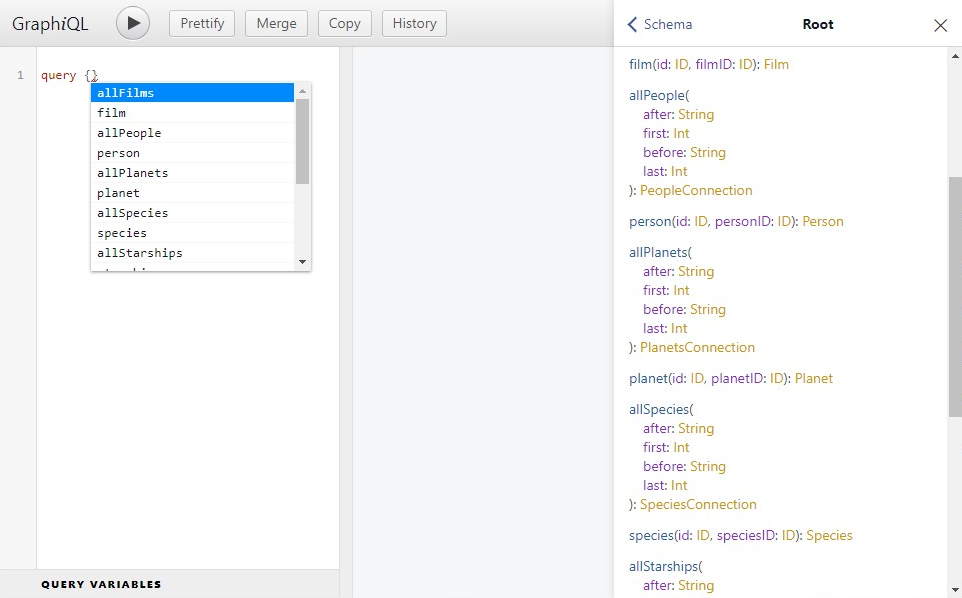
\includegraphics[width=\textwidth]{images/graphiql-autocomplete.png}
    \caption{GraphiQL using Introspection to Generate Auto-Completion Assistance}\label{img:graphiql-introspection}
\end{figure}

This feature of GraphQL can be used to enable developer tools and code generators to query information about the defined type system~\cite{Touronen2019}.
\autoref{img:graphiql-introspection} shows a screenshot of the web-based tool GraphiQL using introspection to programmatically generate human-readable documentation of the \ac{API} as shown on the right-hand side, but also allow developers to write and execute queries against the \ac{API}.
On the left-hand side, developers can write queries and are assisted with auto-completion.
After executing a query, the result will be shown in the middle.

\subsubsection{Schema Stitching and Apollo Federation}

In microservice architectures, a common pattern is using an \ac{API} gateway, providing the client-facing \ac{API}, aggregating data, and routing requests to microservices~\cite{Taibi2018, Touronen2019}.
While such a gateway can be implemented very easily when only \ac{HTTP} requests need to be routed to different services as is usually the case in \ac{REST} \acp{API}, the single \ac{HTTP} endpoint for GraphQL \acp{API} complicates employing this practice more.

\begin{figure}[!htb]
    \centering
    \begin{tikzpicture}[
    node distance=0.5cm,
    component/.style = {
        draw,
        rectangle,
        minimum width = 3.5cm,
        align = center,
        minimum height = 1cm
    },
    process/.style = {
        draw,
        rectangle
    },
    functionality/.style = {
        draw,
        circle,
        minimum width = 5mm
    },
    server/.style = {
        draw,
        rectangle
    },
    sline/.style = {
        line cap=round,
        line join=round
    },
    database/.style = {
        draw,
        cylinder,
        shape border rotate=90,
        aspect=0.25,
        text width = 0.5cm,
        minimum height = 1cm,
        align = center,
        cylinder uses custom fill, cylinder body fill=white, cylinder end fill=black!5
    },
    table/.style = {
        draw,
        rectangle,
        minimum width=5mm,
        minimum height=5mm
    }
]

\node [component] (api1) {GraphQL API};
\node [component, right=of api1] (api2) {GraphQL API};
\node [component, right=of api2] (api3) {GraphQL API};

\node[component, below=0 of api1, minimum height=3cm, anchor=north, text depth=2cm] (bs1) {Data Source};
\node[component, below=0 of api2, minimum height=3cm, anchor=north, text depth=2cm] (bs2) {Data Source};
\node[component, below=0 of api3, minimum height=3cm, anchor=north, text depth=2cm] (bs3) {Data Source};

\node[database] at ($(bs1) - (0,5mm)$) {~};
\node[database] at ($(bs2) - (0,5mm)$) {~};
\node[database] at ($(bs3) - (0,5mm)$) {~};

\node[component, above=1cm of api2, minimum width=11.5cm] (stitching) {Schema Stitching Gateway};
\node[component, above=0 of stitching, minimum width=11.5cm] (api) {GraphQL API};
\node[component, above=of api, minimum width=11.5cm] (client) {Client};

\draw[->] (api) -- (client);
\draw[->] (api2) -- (stitching);
\draw (api1) |- ($(api2)!.5!(stitching)$);
\draw (api3) |- ($(api2)!.5!(stitching)$);


\end{tikzpicture}
    \caption{\ac{API} Gateway for multiple GraphQL \acp{API}~\cite{Touronen2019}}\label{fig:graphql-gateway}
\end{figure}

In practice this problem has been solved in two different ways~\cite{Touronen2019}.
The first option is to simply use \ac{REST} instead of GraphQL at the microservice layer.
The \ac{API} gateway then can expose the combined \acp{API} of the \ac{REST} microservices as a single queryable GraphQL graph.
This strategy usually also is preferred, when legacy microservices need to be integrated into the GraphQL \ac{API}.
The second option combines multiple GraphQL schemas into one.
This can either be done top-down, where the gateway is implemented manually, but it is transparent to the microservices that they are part of a larger \ac{API}, or bottom-up, where the schema of the microservices is annotated with GraphQL directives and the generation of subqueries and routing of requests to the microservices is done automatically based on these directives.
The top-down approach is referred to as \textit{schema stitching} and the bottom-up approach is called \textit{Apollo Federation}~\cite{Stubailo2017,Stuenkel2020}.
However, apart from these differences both schema stitching and Apollo Federation are very similar in functionality and architecture.
\autoref{fig:graphql-gateway} shows the architecture that is employed for both techniques.

As mentioned above, Apollo Federation is implemented using GraphQL directives, that are defined in its specification~\cite{MDGa}.
The core idea of federation is to allow separation of concern for multiple services instead of type-based separation.
Such a type-based separation is exemplarily shown in \autoref{lst:graphql-type-separation}.
This kind of separation, however, has the downside that services need to know about fields of a type, that semantically concern other services.
In the example, the field \texttt{recentPurchases} of the \texttt{User} type is more a concern of the product service than the user service, but must be defined there.

\begin{lstlisting}[language=graphqls, caption={Type-based Separation in GraphQL Schemas~\cite{MDG}}, label={lst:graphql-type-separation}]
# User service --------------------------------------------------------
type Query {
    ~me: ~User
}

type User {
    id: ID
    name: String
    reviews: [~Review]
    recentPurchases: [~Product]
}

# Product service -----------------------------------------------------
type Product {
    id: ID
    name: String
    price: String
    reviews: [~Review]
}

# Review service ------------------------------------------------------
type Review {
    id: ID
    body: String
    author: ~User
    product: ~Product
}
\end{lstlisting}

Apollo Federation allows to separate the types based on concern and implements a variant of multi-view modelling~\cite{MDG, Stuenkel2020}.
Every service can have a different view on the models that concern its functionality.
The same schema using Apollo Federation would look as shown in \autoref{lst:graphql-concern-separation}.
As can be seen, Apollo Federation introduces the additional keyword \texttt{extend}, that has the semantics of not defining a new type, but adding fields to a type of a different service~\cite{MDG}.
Due to limitations of some GraphQL implementations, the \texttt{@extends} directive can alternatively be used on the type.
The \texttt{@key} annotation defines a list of fields that uniquely identify an entity of the given type.
This example also shows, that every service has a different view on the types in the model of other services.
The user service on the one-hand side does not have any information about the existence of products or reviews, while the review service on the other-hand side knows about both model types, but sees only fields relevant to its concern.
Fields that a different service defines, but the using service needs must be annotated with the \texttt{@external} directive to indicate that this is not a duplicate definition of the same field.


\begin{lstlisting}[language=graphqls, caption={Concern-based Separation with Apollo Federation~\cite{MDG}}, label={lst:graphql-concern-separation}]
# User service --------------------------------------------------------
extend type Query {
    ~me: ~User
}

type User @key(fields: "id") {
    id: ID
    name: String
}

# Product service -----------------------------------------------------
type Product @key(fields: "id") {
    id: ID
    name: String
    price: String
}

extend type User @key(fields: "id") {
    id: ID @external
    recentPurchases: [~Product]
}

# Review service ------------------------------------------------------
type Review @key(fields: "id") {
    id: ID
    body: String
    author: ~User
    product: ~Product
}

extend type User @key(fields: "id") {
    id: ID @external
    reviews: [~Review]
}

extend type Product @key(fields: "id") {
    id: ID @external
    reviews: [~Review]
}
\end{lstlisting}

Additionally the \texttt{@provides} and \texttt{@requires} directives are available~\cite{MDGa}.
The \texttt{@provides} directive indicates, that certain fields are guaranteed to be available at a service that does not own the type.
The \texttt{@requires} directive indicates, that although a field may not be required for the query, it is needed in the internal subqueries to a service.
For example consider \autoref{lst:graphql-provides-requires} as part of the review service of the above example: the \texttt{@provides} directive on the \texttt{product} field of the \texttt{Review} type indicates that the product returned by this field will be able to provide its \texttt{name} field, although the type is not owned by the service.
Similarly, the \texttt{@requires} directive on the \texttt{reviews} field of the \texttt{User} type indicates, that the user's \texttt{name} field must be available for the review service to be able to resolve the return value of the \texttt{reviews} field.

\begin{lstlisting}[caption={\texttt{@provides} and \texttt{@requires} Directives of Apollo Federation~\cite{MDG}}, language=graphqls, label={lst:graphql-provides-requires}]
type Review @key(fields: "id") {
    product: ~Product @provides(fields: "name")
}

extend type User @key(fields: "id") {
    id: ID @external
    name: String @external
    reviews: [~Review] @requires(fields: "name")
}

#extend type Product @external { name: String @external }
\end{lstlisting}

Additionally to extensions of the schema, Apollo Federation provides fields on the query type to query the complete schema definition of the services, but also entities of the service~\cite{MDGa}.
Considering the query in \autoref{lst:graphql-federated-query} was received by the gateway, a query plan would be generated that first queries the \texttt{me} field of the query type provided by the user service, selecting only the \texttt{name} field of the returned \texttt{User} object.

\begin{lstlisting}[caption={Query to a Federated GraphQL \ac{API}~\cite{MDG}}, language=graphql, label={lst:graphql-federated-query}]
query {
    me {
        name
        reviews {
            body
            product { name price }
        }
    }
}
\end{lstlisting}

Second, a query to the reviews service would be generated.
This query uses the automatically generated \texttt{\_entities} field on the query type of the service.
This field accepts an array of representations of entities that correspond to the external model and returns the entities corresponding to the local model.
On this query, the result of the previous query would be supplied as an argument and the field \texttt{body} and the \texttt{product \{ id \}} field, to uniquely identify the \texttt{Product} type of the product service.
Lastly, the fetched products of the previous query would be used as representations to query the \texttt{\_entities} field of the product service and select the field \texttt{name} and \texttt{price}.
The result can then be incorporated in the previous query results and the overall result is returned to the user.

\subsubsection{Tools for GraphQL}


\paragraph{GraphiQL}

GraphiQL\footnote{\url{https://github.com/graphql/graphiql}} is a web-based \ac{IDE} for GraphQL \acp{API}.
It provides features such as syntax highlighting for GraphQL queries, auto-completion based in schema introspection, and executing queries against a GraphQL endpoint.
It is developed in Typescript under an open-source license and maintained by the GraphQL Foundation.
It is commonly hosted alongside public GraphQL \acp{API}, for example for the \acp{API} of GitHub\footnote{\url{https://developer.github.com/v4/explorer/}} or Deutsche Bahn\footnote{\url{https://bahnql.herokuapp.com/graphql}}.


\paragraph{GraphQL Playground}

GraphQL Playground\footnote{\url{https://github.com/graphql/graphql-playground}} also is a \ac{IDE} based on GraphiQL.% checktex 13
It provides more powerful features, such as supporting GraphQL subscriptions, specifying \ac{HTTP} headers, or support for inspection of Apollo Federation query plans.
It also is developed under an open-source license and maintained by the GraphQL foundation, but unlike GraphiQL is meant more for local development.

\paragraph{Apollo}

Apollo is a platform for building GraphQL \acp{API} maintained by Apollo Graph Inc..
The core of the platform is Apollo Server\footnote{\url{https://www.apollographql.com/docs/apollo-server/}}, an open-source server implementation of GraphQL.% checktex 13
When combined with Apollo Federation\footnote{\url{https://www.apollographql.com/docs/federation/}}, it can act as an \ac{API} gateway for GraphQL services.
It can also integrate with Apollo Studio, which can be used to gather information about the queryable data graph.
Lastly, Apollo also provides libraries for building GraphQL clients for JavaScript, Android and iOS.% checktex 13

\paragraph{GraphQL Code Generator}

GraphQL Code Generator\footnote{\url{https://graphql-code-generator.com/}} can generate code from GraphQL schemas in different programming languages.
It supports generating both client and server code for different programming languages.
Popular programming languages such as Java, TypeScript, and C\# are supported out-of-the-box, but support for other languages can be added with plugins.

\paragraph{GraphQLJavaGen}

GraphQLJavaGen\footnote{\url{https://github.com/Shopify/graphql_java_gen}} is a Ruby Gem that can be used to generate Java source code for building GraphQL queries and parse the responses for a specific schema.
It works heavily with Java's lambda expressions, which allows writing queries in a similar format to native GraphQL queries.
The generated code, however, does not implement any transport functionality.
This makes customizing \ac{HTTP} requests --- for example, to add authorization headers --- easy because any \ac{HTTP} library can be used.